
%Copyright (C) 2016 by Krishneel@JSK Lab, The University of Tokyo

\documentclass{standalone}
\begin{document}

\subsection{Platforms}
For task 3, we used two types of UAVs for the task. The general UAV called "hawk" as shown in Fig.\ref{fig:task3-hawk}, which is similar to the one used in task 1, and the transformable multilink aerial robot, which is called "Hydrus" (Fig.\ref{fig:task3-hydrus}). As described in Fig.\ref{fig:task3-hydrus-platform}, the hardware platform of "Hydrus" involves the controller for the joints, which enables stable aerial transformation.

\begin{figure}[h]
  \begin{center}
    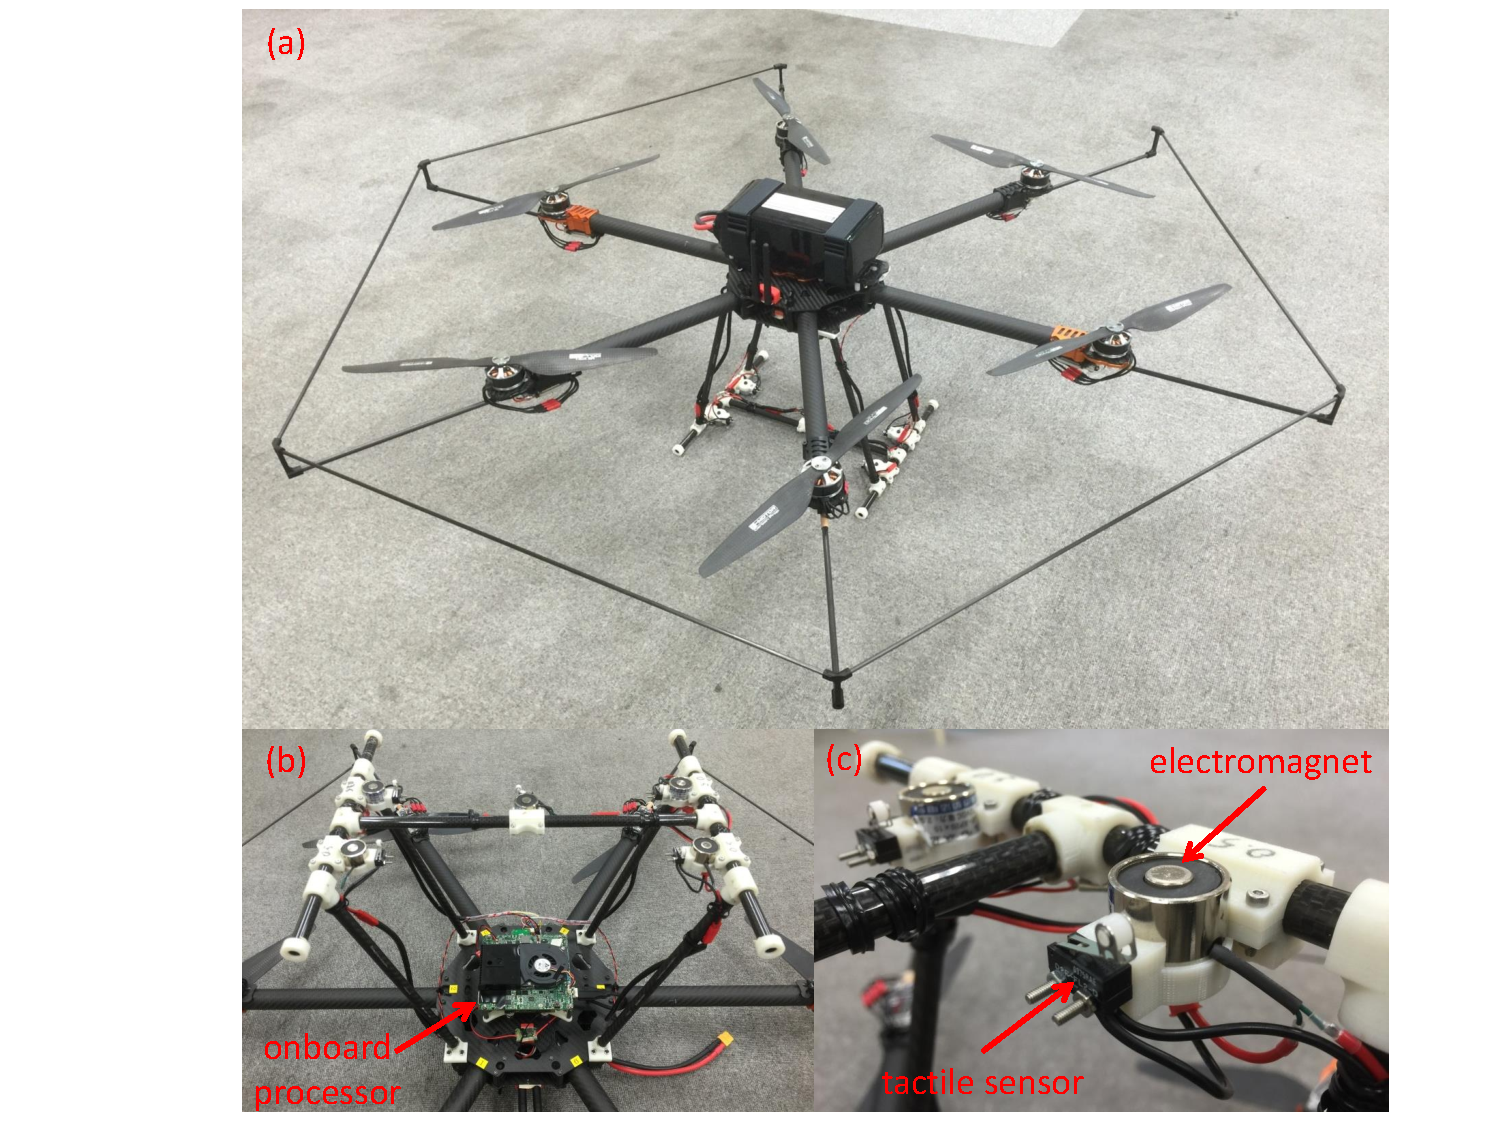
\includegraphics[clip,  bb=115 4 666 535,  width=\columnwidth]{sections/task3/images/task3-tarrot810.pdf}
    \caption{Image of task 3 Hawk}
    \label{fig:task3-hawk}
  \end{center}
\end{figure} 

\begin{figure}[h]
  \begin{center}
    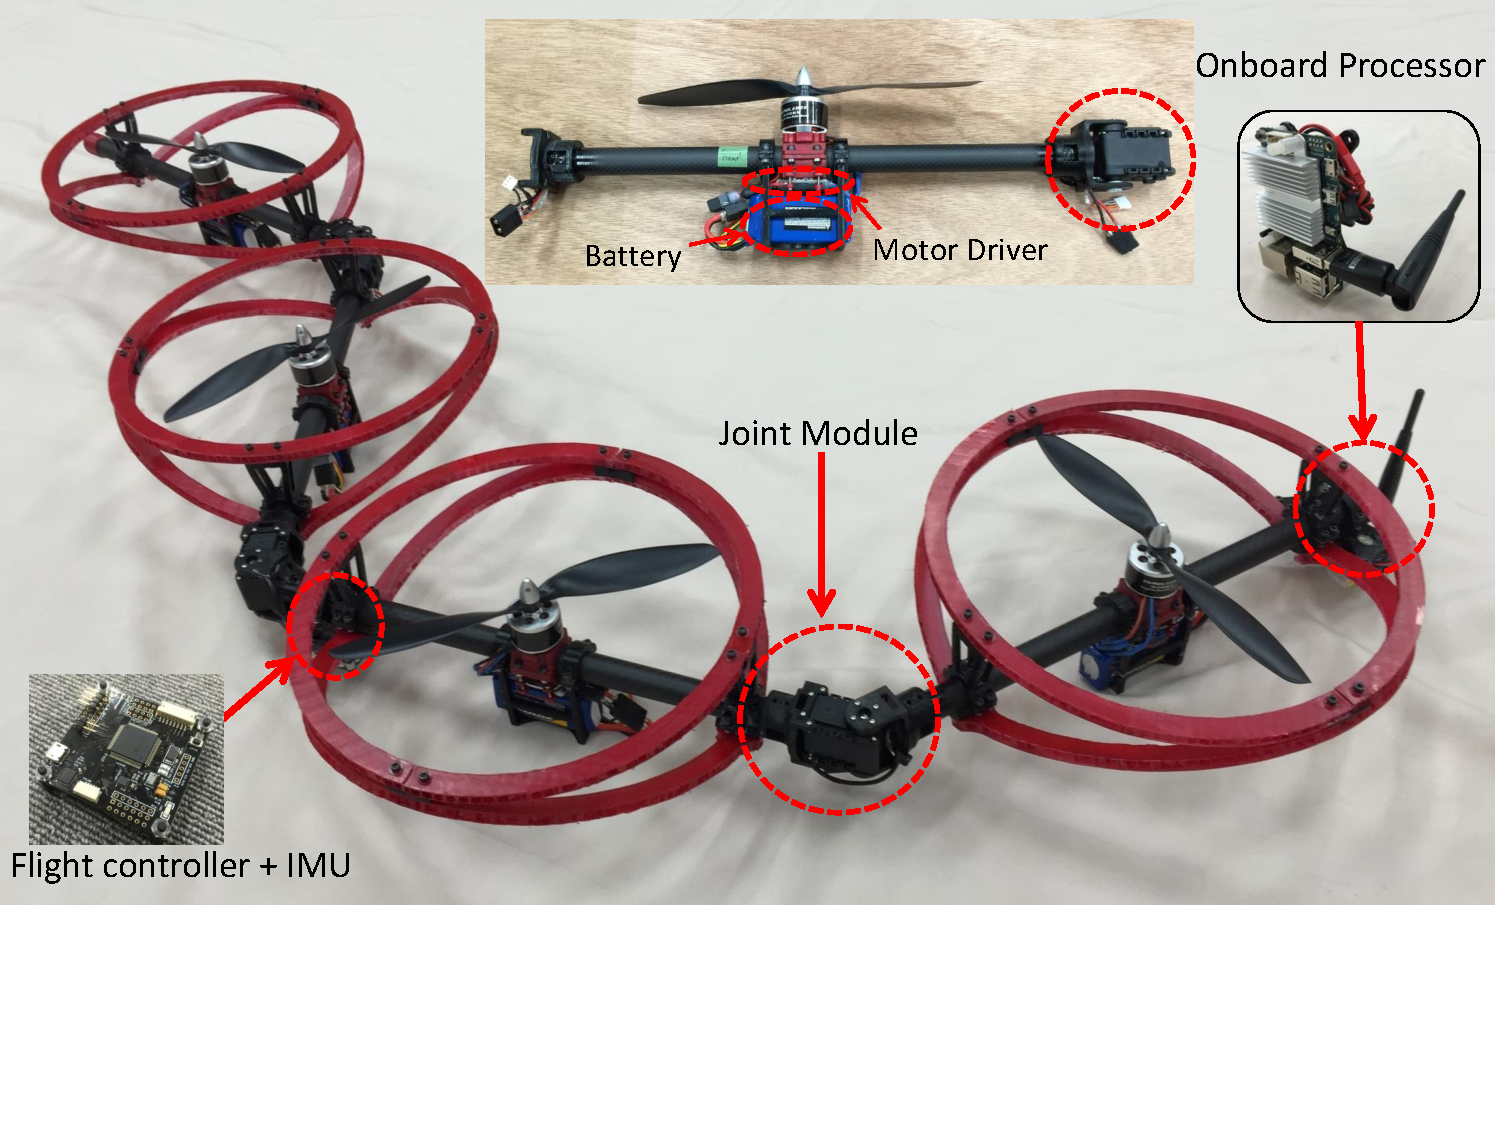
\includegraphics[clip,  bb=0 105 720 535,  width=\columnwidth]{sections/task3/images/task3-hydrus.pdf}
    \caption{Image of Hydrus}
    \label{fig:task3-hydrus}
  \end{center}
\end{figure} 

\begin{figure}[h]
  \begin{center}
    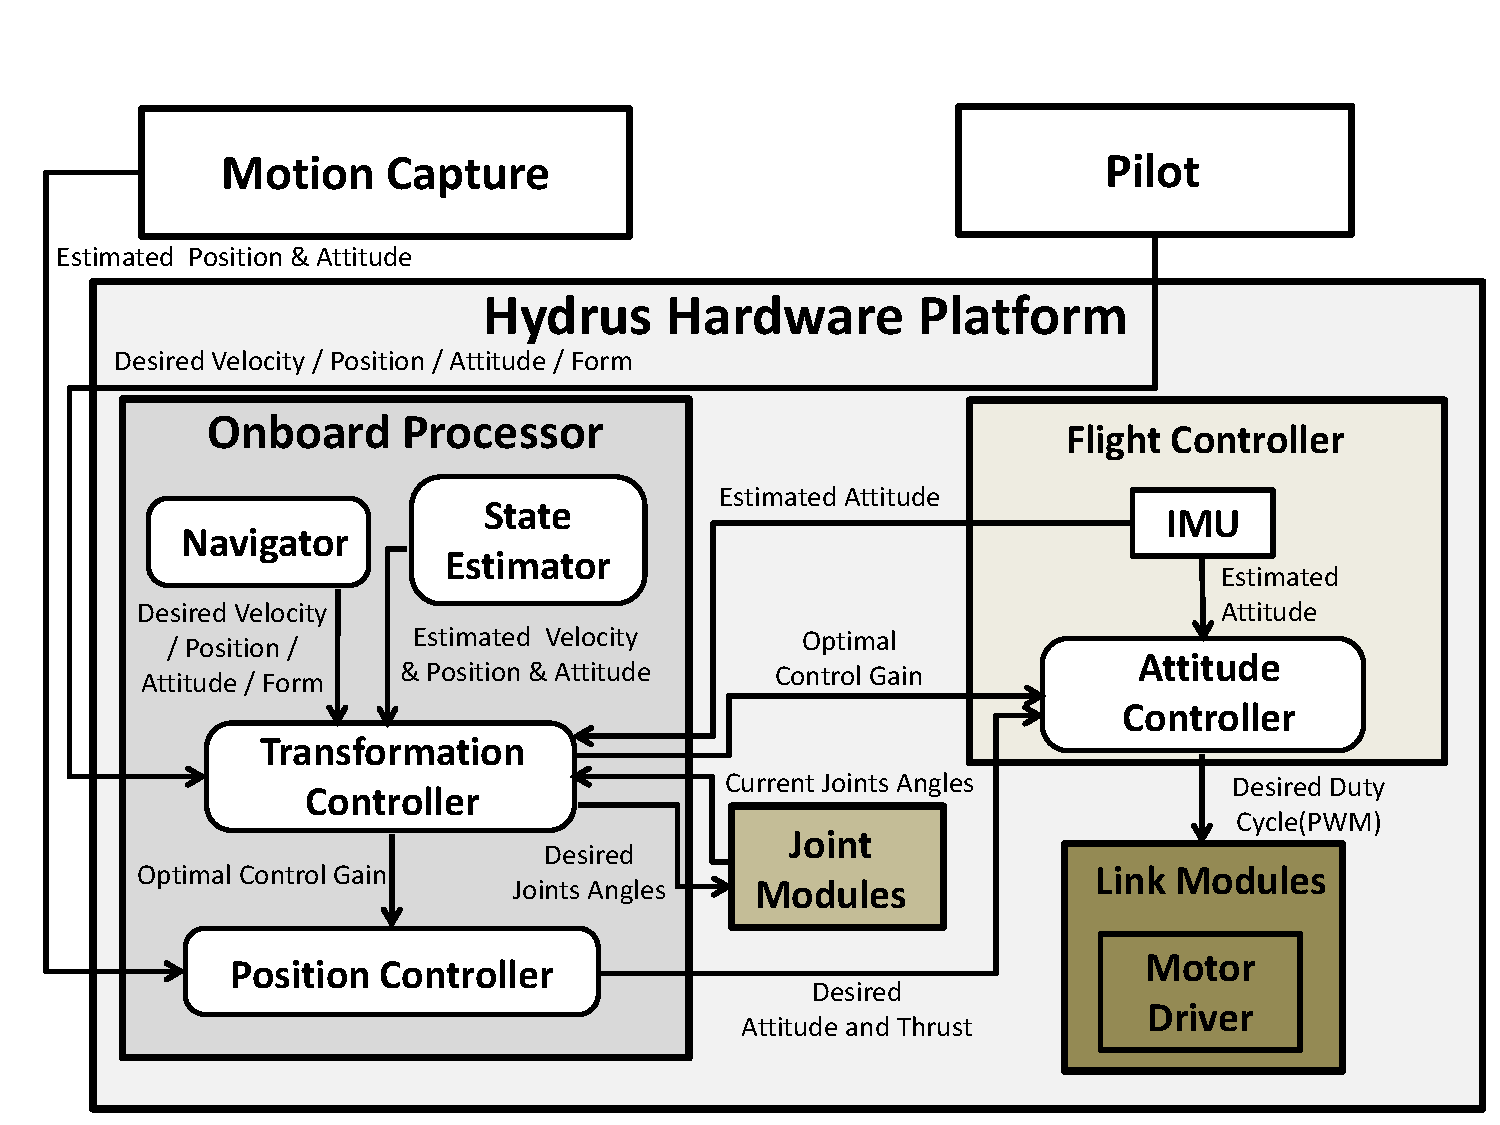
\includegraphics[clip,  bb=0 0 720 540,  width=\columnwidth]{sections/task3/images/hydrus-platform.pdf}
    \caption{Hardware platform of task 3 Hawk}
    \label{fig:task3-hydrus-platform}
  \end{center}
\end{figure} 



Although the flight control algorithms between "Hawk" and "Hydrus" are fundamentally different, we use the same flight controller board which is build by ourselves. For "Hawk", we additionally designed another PCB board for controlling an electromagnet module that can generate attractive forces up to 20[N]. We equipped 5 electromagnets to the UAV and build the attachment with tactile sensors as shown in Fig.\ref{fig:task3-hawk}(c). The electromagnet module control board is connected to the flight  controller board unit through CAN bus.

For the transformable UAV, we introduce the prototype which contains four links and three servo joints. The modularization of the whole platform is achieved by distributing the power and control system to each link with exception to the flight controller and sensors. Therefore, it becomes easier to the change the speed of the rotors for controlling flight.

\subsection{Aerial Manipulation Strategy}
For each type of UAV, we develop a different picking method. For "Hawk" type UAV, we apply magnetic force to attract the ferrous object as shown in Fig.\ref{fig:task3-hawk-manipulation}. When contact between the bottom of the landing gear and the object is detected by the tactile sensors, the electromagnet module is activated. We successfully picked and carried the object in an indoor environment with the use of a motion capture system, validating the electromagnet based manipulation strategy.

\begin{figure}[h]
  \begin{center}
    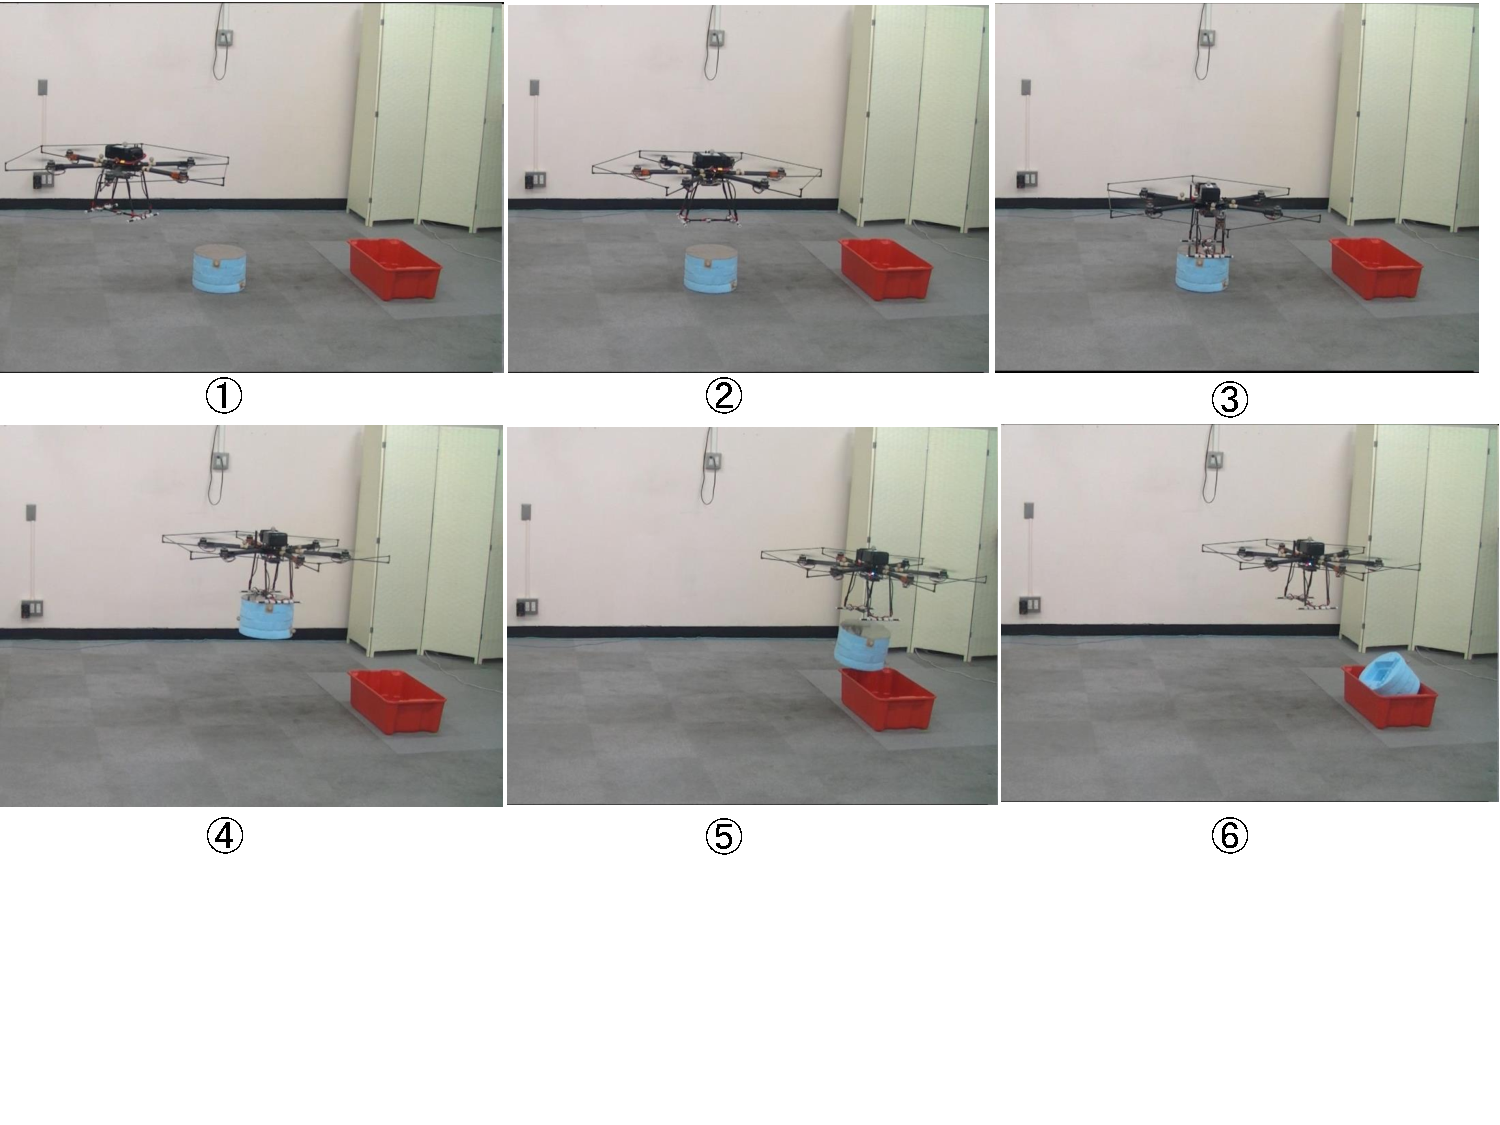
\includegraphics[clip,  bb=0 110 720 540,  width=\columnwidth]{sections/task3/images/task3-tarrot810-manipulation.pdf}
    \caption{Aerial manipulation method of Hawk}
    \label{fig:task3-hawk-manipulation}
  \end{center}
\end{figure} 

Object transportation based on the whole-body-manipulation strategy using "Hydrus" has also been achieved as shown in Fig.\ref{fig:task3-hydrus-manipulation}. Grasp control is achieved based on torque feedback from each joint. 

\begin{figure}[h]
  \begin{center}
    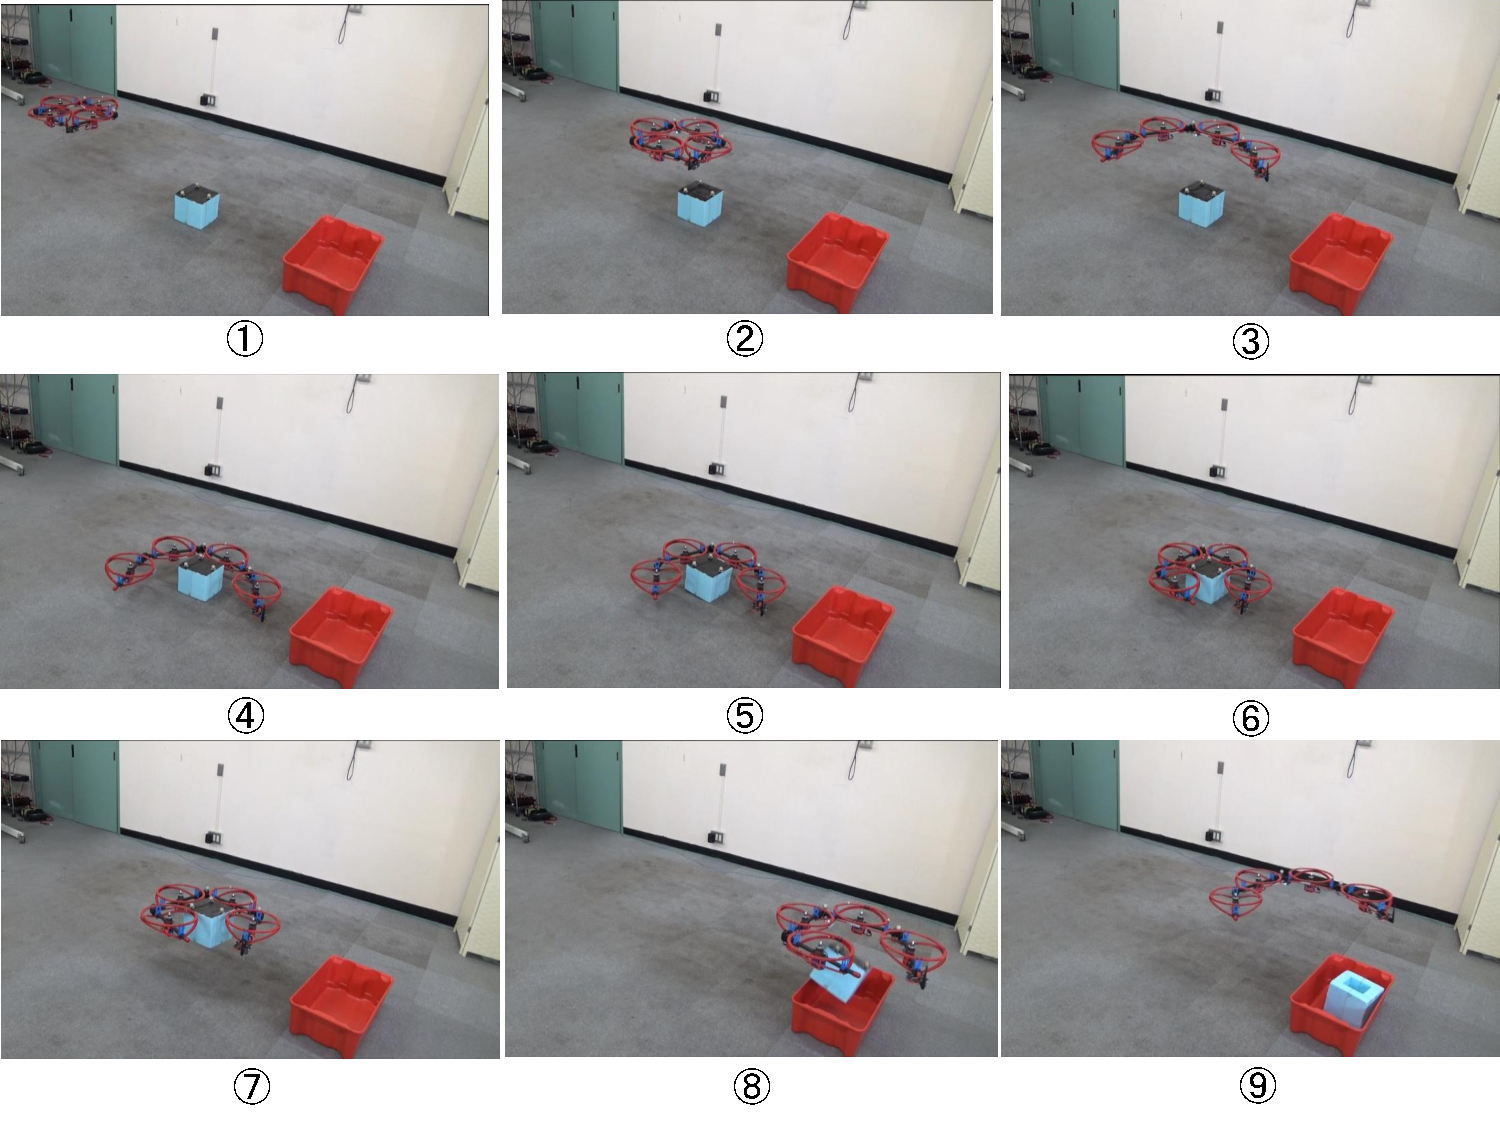
\includegraphics[clip,  bb=0 0 720 540,  width=\columnwidth]{sections/task3/images/task3-hydrus-manipulation.pdf}
    \caption{Aerial manipulation method of Hydrus}
    \label{fig:task3-hydrus-manipulation}
  \end{center}
\end{figure} 


\subsection{Software}
As with other tasks, the software is build using ROS and some functionalities are shared with task 1. Point Cloud and OpenCV libraries are used for visual perception. % target detection and motion planning are different.


\subsection{General Approach}
%The software system is based on ROS(Robot Operation System). We write our algorithm to the every single node and communicate with each node. 
\subsubsection{Overall Strategy}
We divide the task into three states: Search, Pick, and Place. The UAVs are always in one of these three states and the states automatically transition into the next one when certain conditions are met as illustrated in Fig. \ref{t3}A. In the "Search" state, the drone will traverse to the center of the arena and randomly generate a search end-point, the treasure detector will run while the drone is searching. Once the object is detected and locked, a pick motion will be generated. In the "Pick" state, the UAV will turn on the electromagnet and approach the treasure (for $Hawk$) or enclose its body around the treasure (for $Hydrus$). The state transition from the "Pick" state is signalled by the triggering of the tactile sensor. Once the electromagnet of the $Hawk$ has caught the treasure or the body of the $Snake$ has enclosed the treasure, the UAV transitions into the next state. In the "Place" state, the UAV will fly directly to the placing zone and find the box to place the treasure in. After releasing the treasure into the place box, the UAV re-enters the "Search" state and loops until the task is completed.

 \begin{figure}%[hb]
    \begin{center}
      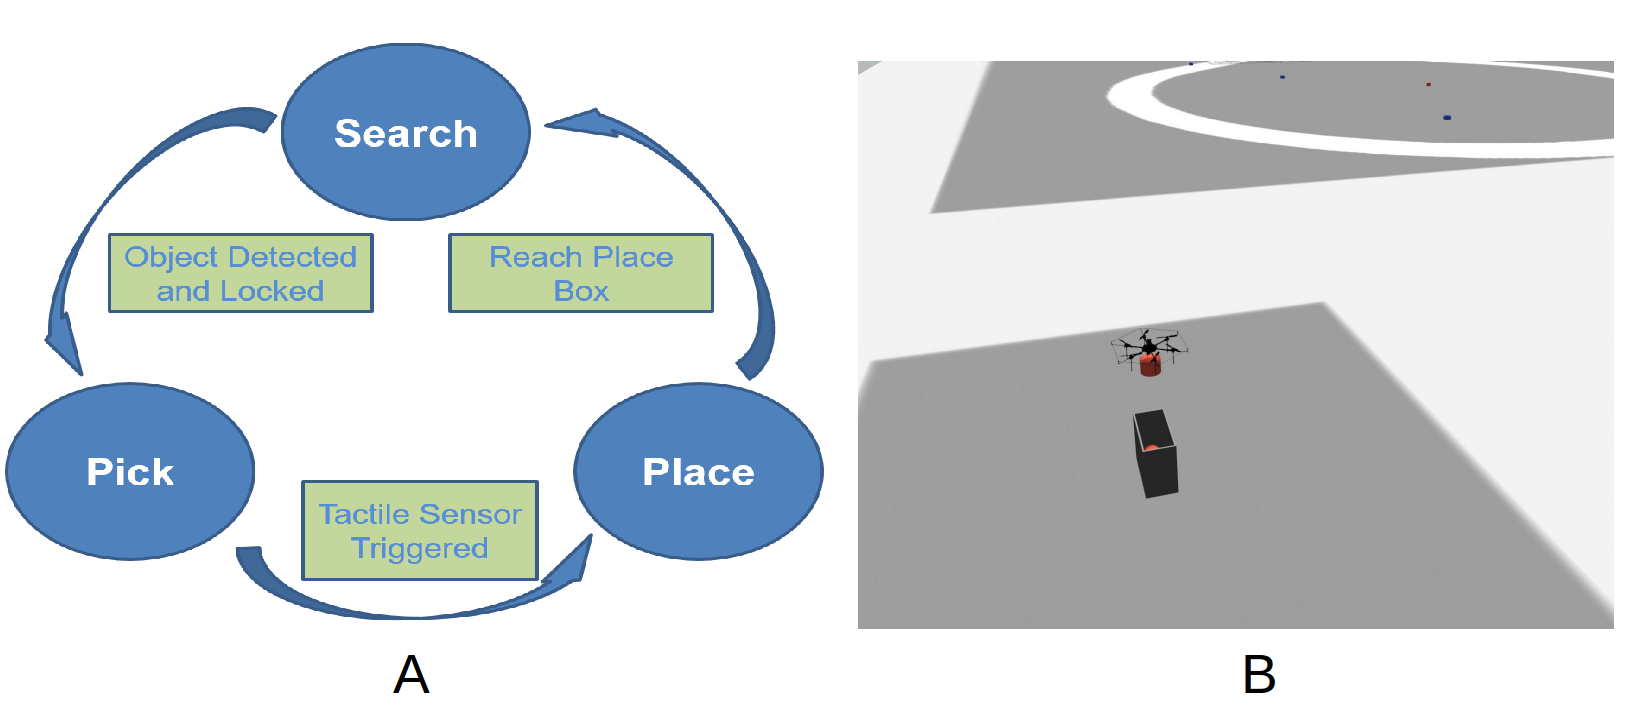
\includegraphics[keepaspectratio=true, width=1\linewidth, height=0.30\textheight]{img//task3.png}
    \end{center}
    \caption{Task 3 Demonstration}
    \label{t3}
  \end{figure}


\subsubsection{Treasure Detection}
As the treasures have distinct color features, we first used a simple detection method to detect the treasures. 
The inputs are 3D points $p_i$ from the stereo sensor and the RGB image projection onto the ground by the projection matrix computed using the known camera parameters. %We first apply 
HSI color filter is applied to obtain the 3D point candidates of the treasures from the point cloud data. Next, we apply Euclidean clustering to the filtered point cloud $P_{hsi}$. Euclidean clustering technique can organize points into clusters with respect to distance features in 3D space. For $\forall p_i, p_j \in P_{hsi}$, clusters $O_i = \{p_i \in P_i\}$ and $O_j = \{p_j \in P_j\}$ are obtained by:
\begin{equation}\label{eq3-1}
min||p_i - p_j|| \geq d_{threhold} 
\end{equation}

After we obtained all the clusters, we apply a simple tracker to every cluster center, and as we continue to detect the same cluster over time, the weight of the tracker is increased to boost the confidence of tracking. For clusters that are not always detected the confidence are slowly decreased and removed from the treasure candidates vector. The UAV will lock on to the cluster candidate when the weight is large enough and switch into the "Pick" mode to approach the treasure.

\subsection{Results Achieved to Date}
We first performed full automatic simulation in Gazebo as shown in Fig.\ref{t3}B. To fully simulate the real scene, we add noise and outliers to the detection. In simulation, the UAV takes almost 70$seconds$ to detect, pick and place a single object. 
% we believe we can do that better. 
With the real robots, we tested tele-operation control, and both the $Hawk$ and the $Snake$ were able to grasp the treasure and pick and place it into a specified box. 

\subsection{Future Plans}
In our next steps, we will use three UAVs in coordination to complete the task which will not only decrease the time but also can be used to transport larger treasures which a single UAV might not be able to lift. We will also be carrying out more experiments on the real robots to test the detection and motion planning algorithm that have been verified in simulation.

Future work on hardware for task 3 includes the improvement of the structural strength, as well as the enhancement of the modularization of link system by using CAN communication network. We will also continue to validate the performance of the electromagnet module, and the integrated use of electromagnetic force and whole-body-manipulation will be developed for "Hydrus".

Future work on software for task 3 involves outdoor experiment with actual robots to test the performance of both electromagnet module and whole-body-manipulation. In addition, we will focus on the collaborative motion for picking up the large object using two or three UAV simultaneously, as well as swarm control strategy while searching object.


\end{document}
